\section{Influence of Skill Orders}
\label{sec:influence}

This project came up from the investigation of the dataset, Assistments, used in the original DKT paper. There are several data ordering issues in Assistments and preliminary results suggest that the structure inside the sequential data could be discovered by investigating the DKTs trained on reordered data. I'm mainly responsible for the project, and Shayan, as an EDM veteran, would also advice me in this project.

\subsection{Data Quality Issues for Assistments Dataset}

The original DKT paper reports a 0.86 AUC on the Assistments dataset, which is the largest public educational dataset so far. However, by closely investigating this dataset, several data quality issues emerge. I independently discovered some of those, while a recent EDM paper\footnote{\textit{Going Deeper with Deep Knowledge Tracing}, Xiaolu Xiong, Siyuan Zhao, Eric G. Van Inwe- gen, Joseph E. Beck, EDM 2016.} has a more comprehensive coverage. Such issues greatly inflate the AUC result of the DKT, which make the reported AUC completely lose its credibility.

Besides trivial misprocessings like keeping the scaffolding problems, there are three major data quality issues. First, a great percentage of the dataset is duplicated, where same record with the same timestamp could be repeated for more than 200 times. This would obviously boost the prediction performance, since the model would observe 200 identical records in a row.

The other two issues, which direct us to launching this project, are more subtle and would be described in the following two sections. 

\subsection{Reordering the Skills}

In the original Assistments dataset, records are not presented in chronological order. Instead, the trajectory is organized in what we call a numerical order, where records of the same skill are grouped together, and the chronological order of results (i.e. correct or incorrect) within a skill is preserved. To better understand the influence of the numerical order, we train on data with one of the order schemes, and test on data with another ordering. As comparison, we add two more reordering schemes. Chronological-shuffle means that we shuffle the order of the skill encountered by the student, yet still keep the chronological order of results within the same skill (like what we did in numerical ordering). The baseline order is random order, which completely shuffles the data without preserving any chronological order. The four order schemes are showcased in figure \ref{fig:4order}.

\begin{figure}
\subfloat[Chronological order]{
  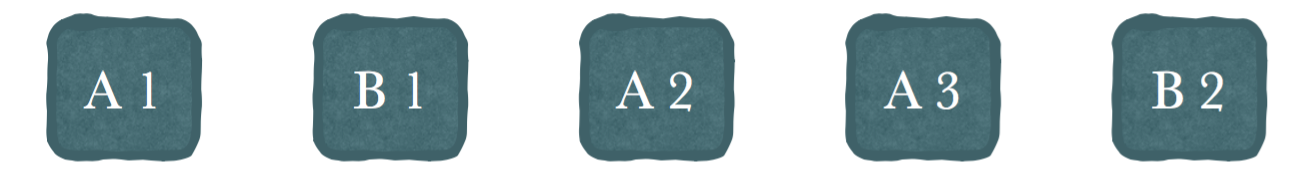
\includegraphics[width=0.45\linewidth]{figures/chronological.png}%
}
\hspace{0.1\linewidth}
\subfloat[Numerical order]{
  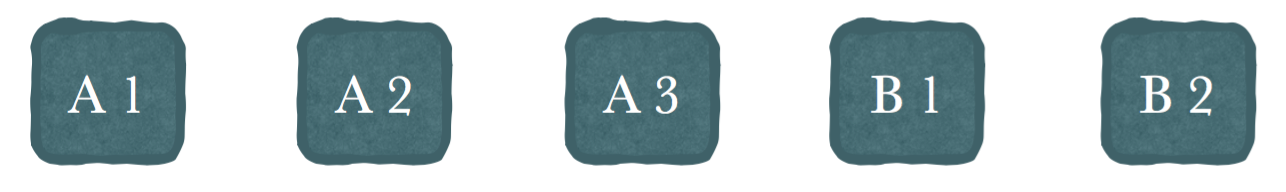
\includegraphics[width=0.45\linewidth]{figures/numerical.png}%
}
\newline
\subfloat[Chronological-shuffle order]{
  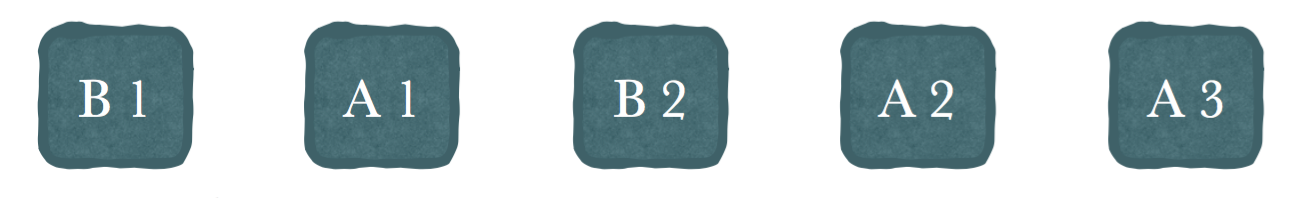
\includegraphics[width=0.45\linewidth]{figures/chronological-shuffle.png}%
}
\hspace{0.1\linewidth}
\subfloat[Random order]{
  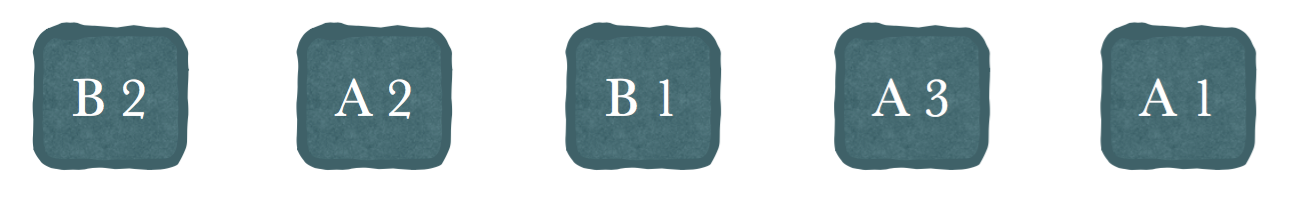
\includegraphics[width=0.45\linewidth]{figures/random.png}%
}
\caption{Four order schemes. Skill A has three records, while skill B has two. The numbers stand for the original(chronological) order within the same skill.}
\label{fig:4order}
\end{figure}

Figure \ref{subfig:assist_repeat} is the initial result we got on the Assistments data, with the performance of training and testing on chronoligical order siginificantly outperforms other order schemes. We can at least draw three conclusions from this result:

\begin{itemize}
\item There is a pattern of knowledge acquisition over time for our model to learn (thus chronological > random). 
\item There is a strong correlation between the acquisition of different skills (thus chronological > numerical).
\item The structure of skill acquisition preserves a bit in numerical order, but would be completely broken down in chronological-shuffle (thus numerical > chronological-shuffle).
\end{itemize}

In a nutshell, the fact that AUC drops significantly after shuffling the skill orders (which simultaneously break the inter-skill structure presented in the data) suggests that we probably could measure skill relations with AUC drops after reordering. This is the decisive result that make us think this project might be promising.

\subsection{Multi-skill Questions}

\begin{figure}
\subfloat[Assistments, repeated scheme]{
  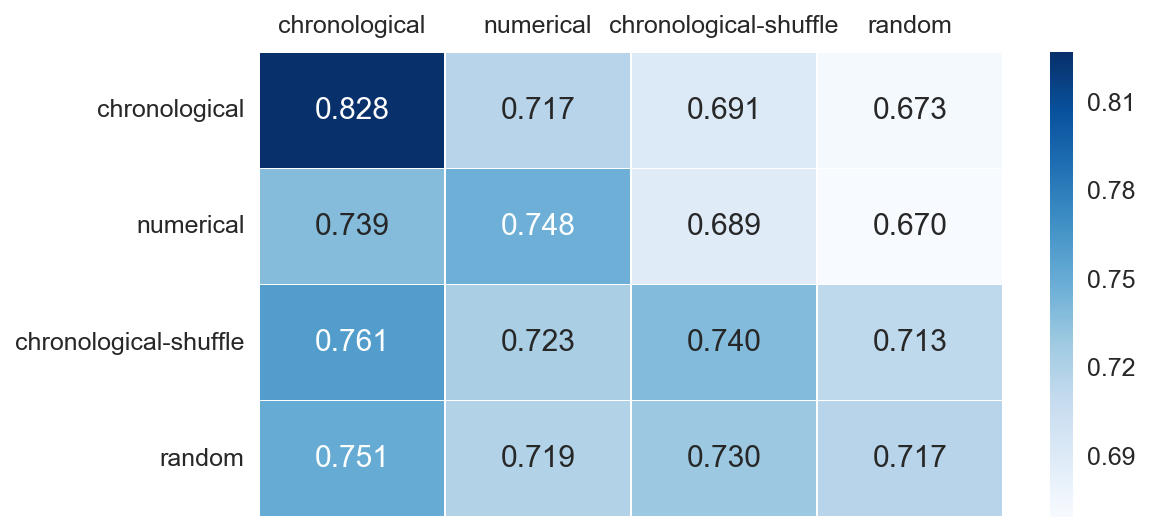
\includegraphics[width=0.5\linewidth]{figures/6th_cross_test_new.png}%
  \label{subfig:assist_repeat}
}
\subfloat[Assistments, joint scheme]{
  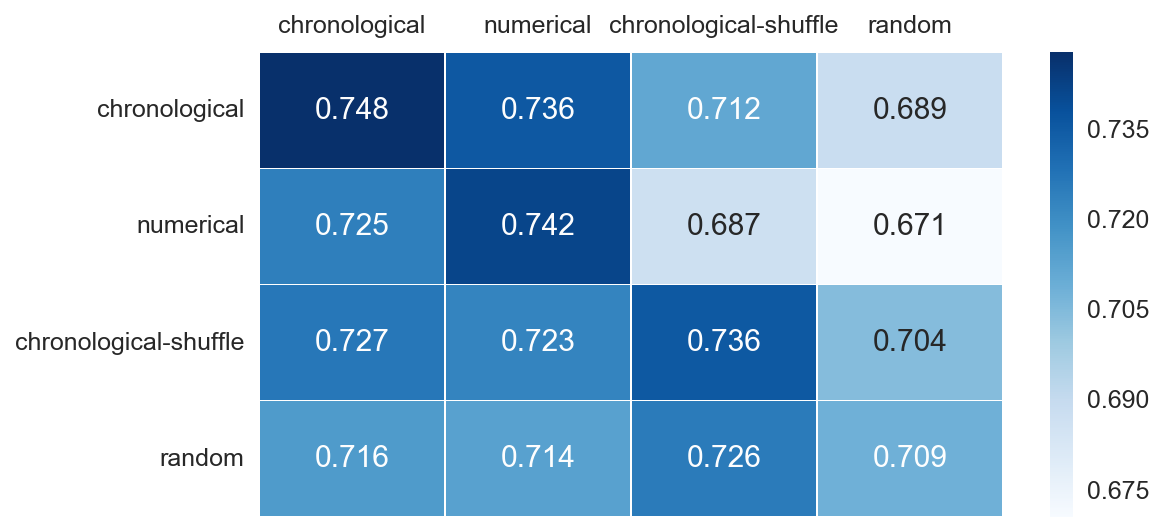
\includegraphics[width=0.5\linewidth]{figures/7th_joint_skill_cross_order.png}%
  \label{subfig:assist_joint}
}
\newline
\subfloat[BKT Simulation]{
  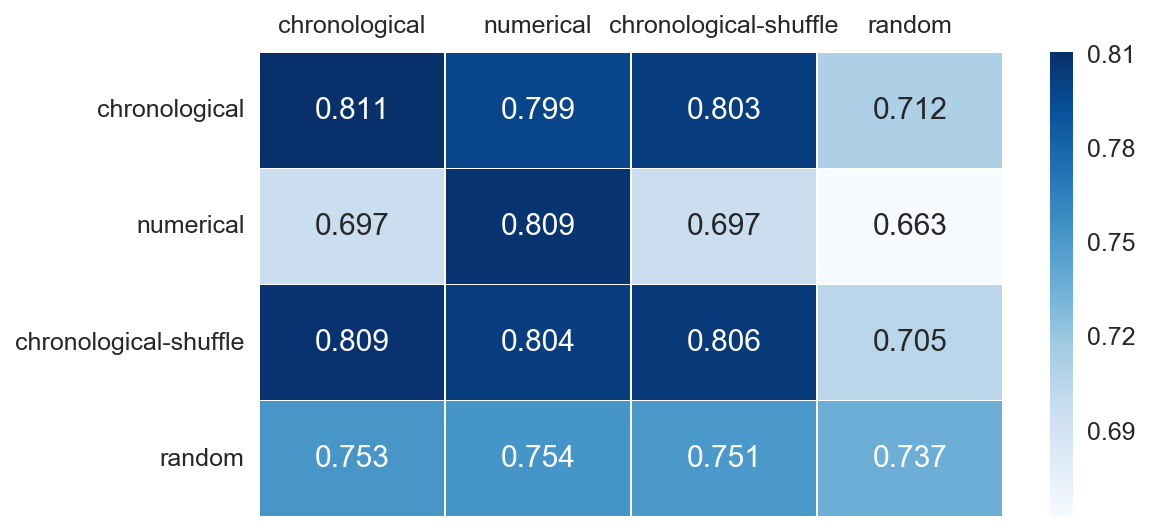
\includegraphics[width=0.5\linewidth]{figures/8th_simulation_cross.png}%
  \label{subfig:bkt_simul}
}
\subfloat[Fraction, 105 skills]{
  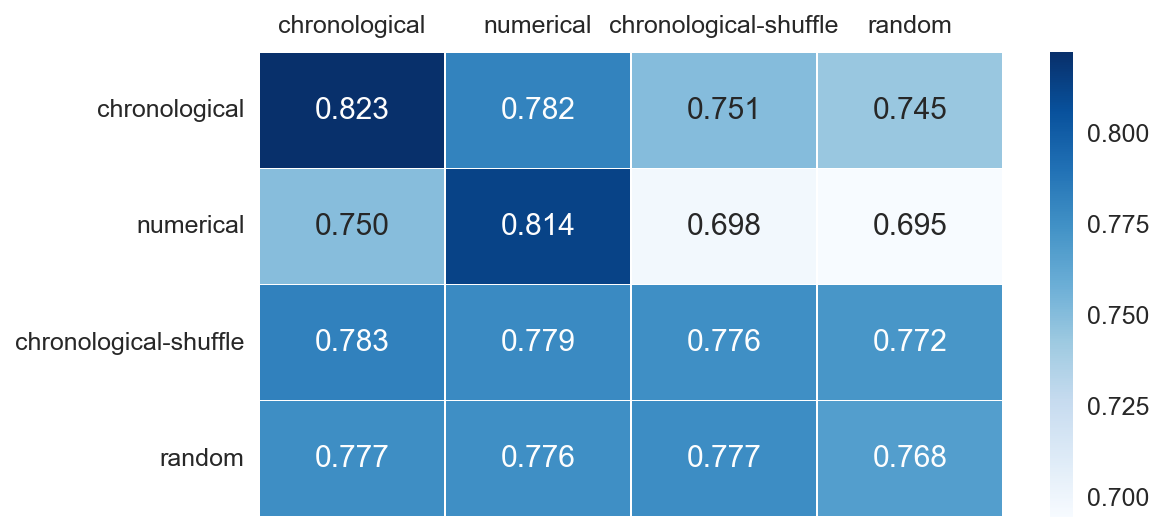
\includegraphics[width=0.5\linewidth]{figures/8th_fraction_cross.png}%
  \label{subfig:fraction}
}
\caption{Reordering test results (AUC of prediction) on four datasets. Row labels are the order of the train set, and column labels are the order of the test set.}
\label{fig:reorder}
\end{figure}

However, a closer look at the data reveals another data quality issue that could severely inflate the prediction AUC.
Some problems in the Assistments dataset are associated with multiple skills. Such problems are presented as multiple consecutive records, each associated with a single skill. Since they are actually one problem, the correctness (result) is same for the records. An example of this repeated scheme can be found in table \ref{tb:repeated}. Such scheme would hint the DKT with the ground truth when DKT takes the first record as an input. For the consecutive records that are actually of the same problem, the result won't change, thus would definitely be correctly predicted. To confirm this, we separately compute the AUC for the repeated records in the test set, and the AUC is over 0.9999, which is basically a perfect prediction.

\begin{table}[]
\centering
\begin{tabular}{|c|c|c|c|}
\hline
Time Stamp & Problem & Skill & Correct \\ \hline
5678       & 100     & 1     & 0       \\ \hline
5678       & 100     & 2     & 0       \\ \hline
5678       & 100     & 3     & 0       \\ \hline
5679       & 101     & 1     & 1       \\ \hline
5679       & 101     & 2     & 1       \\ \hline
5679       & 101     & 3     & 1       \\ \hline
\end{tabular}
\caption{Repeated scheme: repeated records for different skill tags of the same problem.}
\label{tb:repeated}
\end{table}

To resolve this issue, we need to keep only one record for each problem. We can make every skill combination of multi-skill problems a new skill, which is assigned a new skill id, as shown in table \ref{tb:joint}. Under this scheme, we repeat the reorder test and the results are shown in figure \ref{subfig:assist_joint}. We can see that most AUC results don't change much, yet the AUC of train on chronological test on chronological suffers a huge drop, since in this case there won't be a hint to leverage as in the repeated the scheme.

Joint scheme has its own deficiencies, since it completely loses the representation of its components. DKT won't know (at least not explicitly) the sub-skills of a joint-skill, thus might perform worse on predicting other stand-alone records of the sub-skills. We can simply sample one of the skills in the multi-skill question and discard all other records to preserve some of the components of a joint-skill. However, this yields an even worse AUC, since it's only an approximation of the problem.  

\begin{table}[]
\centering
\begin{tabular}{|c|c|c|c|}
\hline
Time Stamp & Problem & Skill & Correct \\ \hline
5678       & 100     & 145   & 0       \\ \hline
5679       & 101     & 145   & 1       \\ \hline
\end{tabular}
\caption{Joint Scheme: one record per problem, with a new skill id.}
\label{tb:joint}
\end{table}

We made a novel modification to DKT, aiming to resolve such dilemma. The new DKT takes a multi-hot encoding of an action as input, where multiple elements in the vector are 1, each corresponds to a sub-skill (while the original DKT takes one-hot encoded inputs). And when making predictions, the DKT multiplies the belief states of sub-skills based on the assumption that a student has to know all the sub-skills to correctly answer a multi-skill question. To our surprise, this still results in the same AUC as the joint scheme. By taking a closer look at the LSTM, we notice that a multi-hot vector won't be treated as a combination of several one-hot vectors in the computation, but more close to a completely new vector. Therefore it's basically equivalent to the joint scheme.

\subsection{Extracting Prerequisite Relations with Reordering}

Though not as significant as figure \ref{subfig:assist_repeat}, we can still observe that training on chronological data holds a clear advantage over other order schemes when tested on chronological data. In order to get a sense of the scale of AUC difference we should be expecting, we conducted the same reordering expriments on the BKT simulation dataset. However, as shown in figure \ref{subfig:bkt_simul}, the result is quite surprising: training on numerical order is way worse, while training on chronological-shuffle order is on par with chronological. 

On Fraction dataset we observed a descent AUC difference between chronological-shuffle and chronological, as shown in figure \ref{subfig:fraction}. We took a closer look by computing the AUC for each skill separately when trained on chronological-shuffle and tested on chronological. In this case, we won't get a correct DKT model, since the relative order of skills is messed-up in the train set. Therefore, only independent skills would keep the same AUC, while skills with either ancestors or children would suffer a big AUC drop. About 20 out of 105 skills suffer a huge AUC drop. This result gives us more confidence on our method.

We tried another way of reordering with the simulation dataset. We train DKT on the chronological ordered data, but when we test it, we completely shuffle the order of one of the skill while preserving the order of other skills. When we investigate the per skill AUC in the test set, obviously the shuffled skill would have the biggest drop. According to figure \ref{fig:drop}, the closer the skill in the hierarchical structure is, the bigger the AUC drop. However, we are expecting AUC drops with bigger values.

\begin{figure}
    \centering
    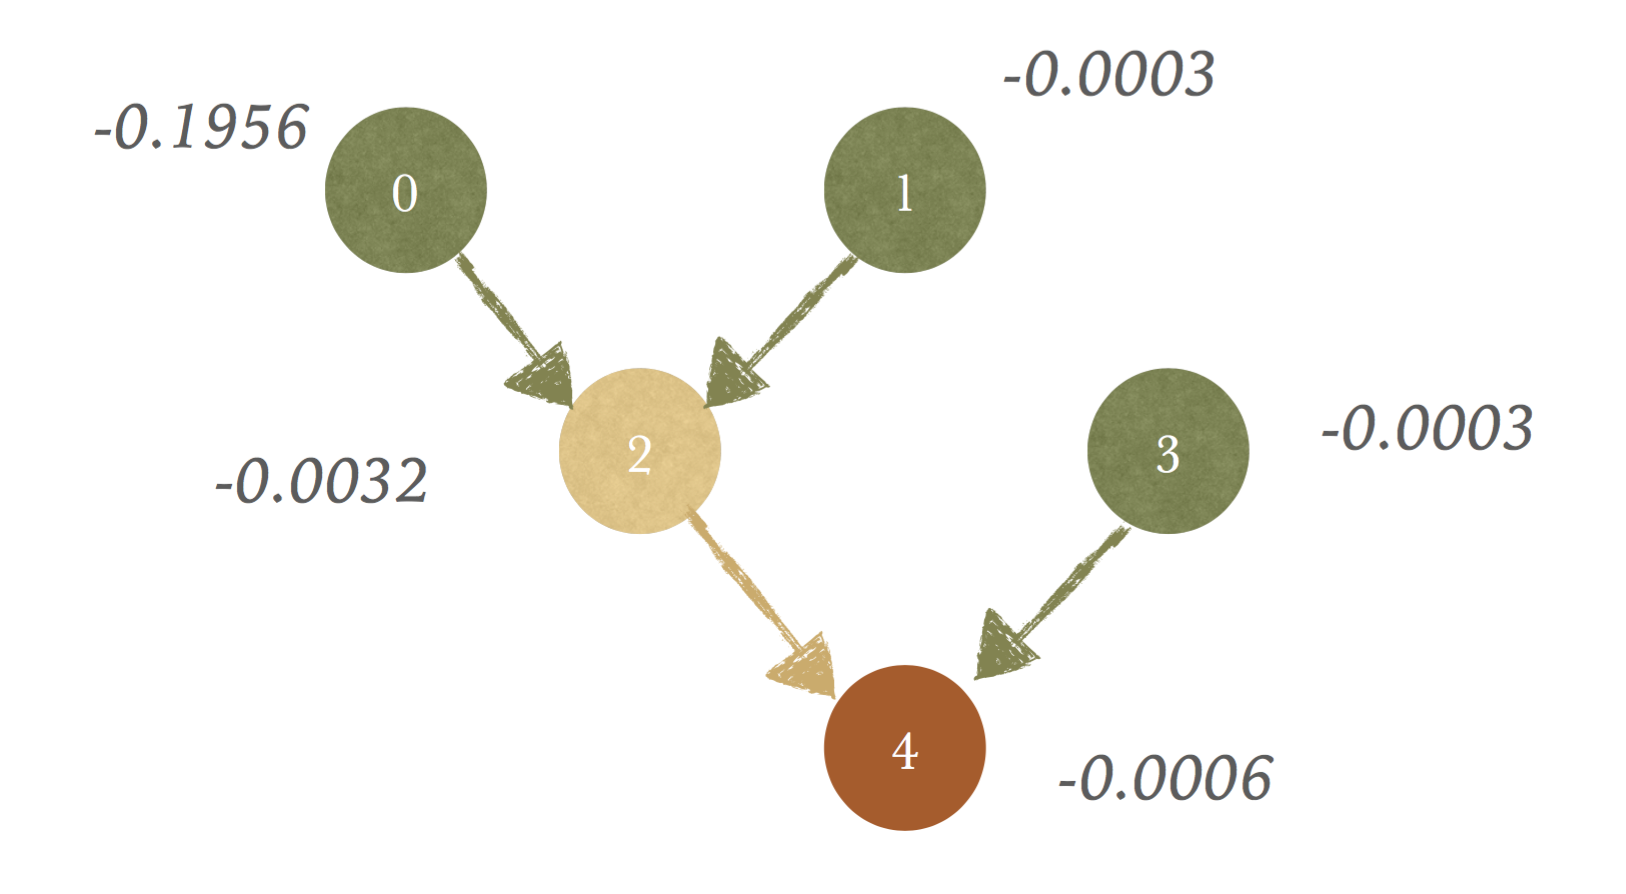
\includegraphics[width=0.6\linewidth]{figures/simulation_AUC_drop.png}
    \caption{The per skill AUC drop on the BKT simulation test set when skill 0's order is shuffled. Skill 2 takes 0 and 1 as prerequisites, while skill 4 takes 2 and 3 as prerequisites.}
    \label{fig:drop}
\end{figure}

\subsection{Future Work}

We decided to write up our findings as a paper. Therefore, besides keeping progressing on the experiments, we also need to start literature search. 

As for the experiments, the priority would be to work out the detailed logistics of extracting knowledge components' relations with reordering. There are several concerns: shuffle a single skill or a group of skills; shuffle the train test or the test set; what threshold to set for filtering the noise. To better investigate these issues, we need to train an interpretable model, i.e. a BKT, so that we can check the learned model by comparing it with the ground truth model used in simulation. Based on this, we will move on to DKT and real world data.

The bizzare results observed in figure \ref{subfig:bkt_simul} also need to be proper explained, since that may lead us to a deeper understanding of sequential data orders and DKT. We have already tried different simulated data with additional attributes like interleaving questions or shifting question distributions to figure out when AUC stays the same after shuffling. However, no conclusion has been reached.

The preliminary literature search suggests several possible advantages of our methods over proposed EDM methods. First, DKT as a deep learning model could capture more subtle skill relations, and unlike many other methods, no domain knowledge is required. As for the only proposed method for extracting skill relations with DKT, it suffers from several deficiencies. This method uses the belief state change of skill $j$ after correctly answering a question on skill $i$ as a metric of the relation between the two skills. Figure \ref{fig:20_in_a_row} shows the tracing results given by DKT when input a trajectory of getting one of the skills correct 20 times in a row. We can see that when a skill's belief state goes up, its prerequisites' belief states would also go up. And after extreme cases like 20 corrects in a row, they would all end up in a near perfect belief.

However, in real world data, such strict prerequisite relations won't exist, thus we couldn't tell if a AUC rise is truely resulted from skill relations. In figure \ref{subfig:skill_1}, the belief for skill 0 goes up as well, but it's independent with skill 1. In real world dataset, such noise would harm the validity of our conclusions. Moreover, the relations between skills might show up after several observations, as shown in figure \ref{subfig:skill_4}. Thus basing our conclusion on only one observation like the proposed method would be too myopic, even for simulated data.

More literature search need to be done to fully motivate and justify our method.

\begin{figure}
\subfloat[Skill 0]{
  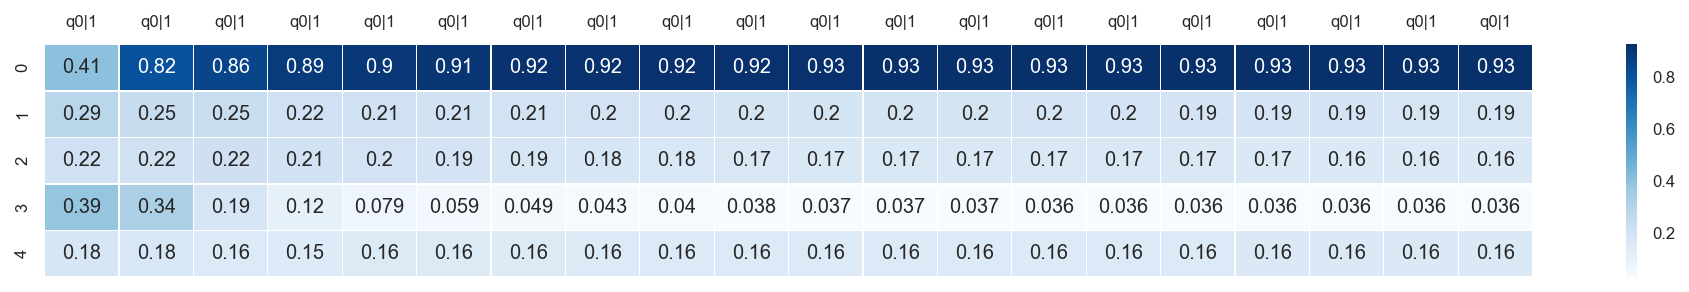
\includegraphics[width=1.0\linewidth]{figures/9th_skill_0.png}%
}
\newline
\subfloat[Skill 1]{
  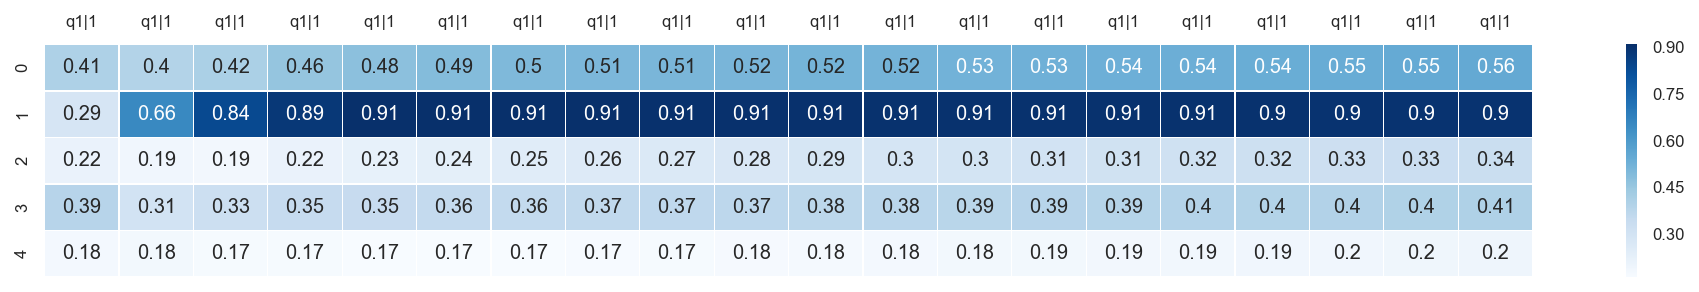
\includegraphics[width=1.0\linewidth]{figures/9th_skill_1.png}%
  \label{subfig:skill_1}
}
\newline
\subfloat[Skill 2]{
  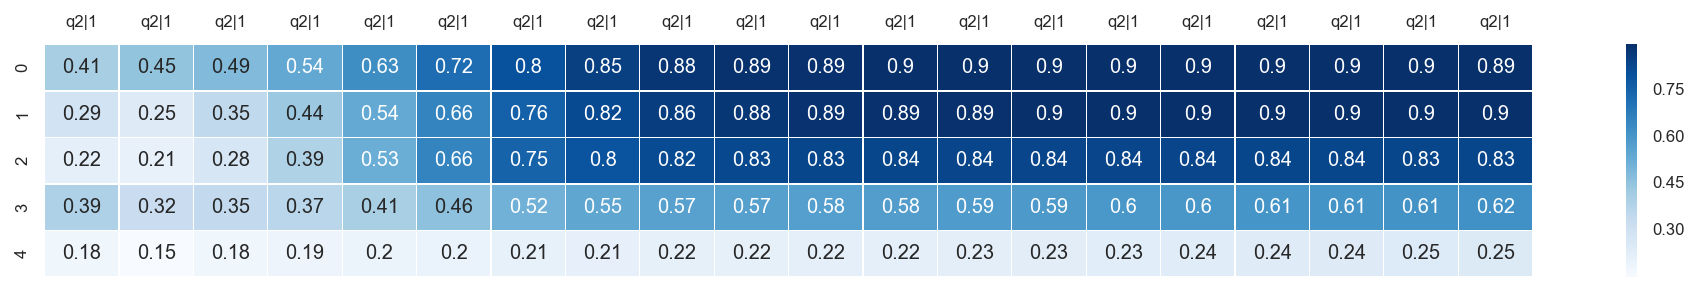
\includegraphics[width=1.0\linewidth]{figures/9th_skill_2.png}%
}
\newline
\subfloat[Skill 3]{
  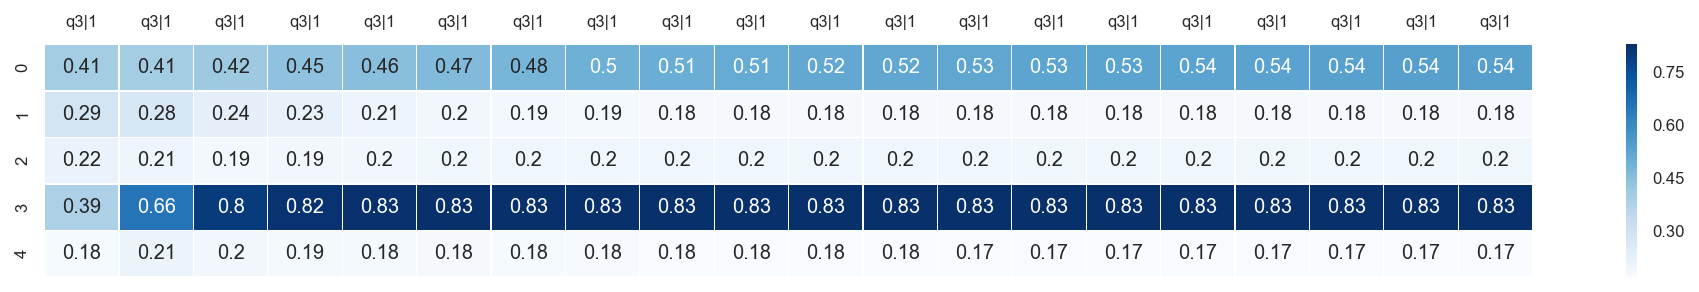
\includegraphics[width=1.0\linewidth]{figures/9th_skill_3.png}%
}
\newline
\subfloat[Skill 4]{
  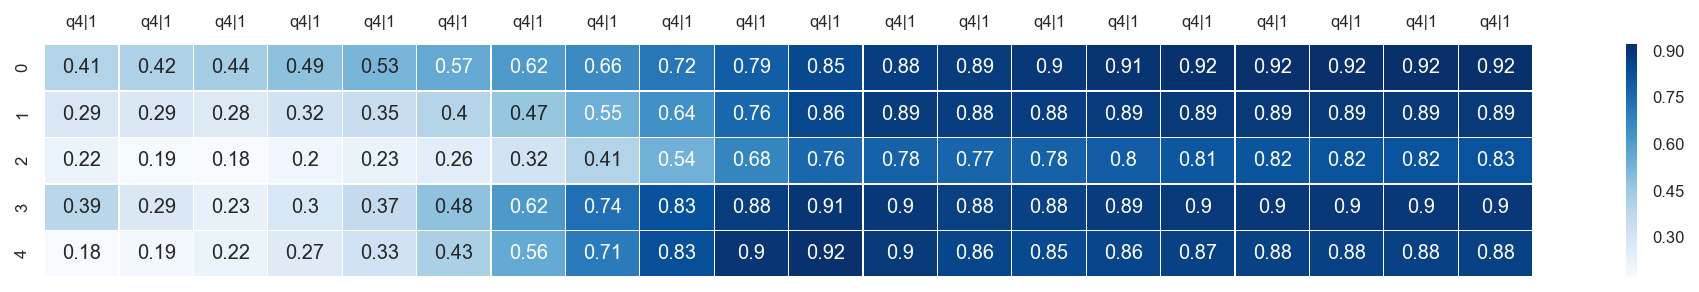
\includegraphics[width=1.0\linewidth]{figures/9th_skill_4.png}%
  \label{subfig:skill_4}
}
\caption{DKT's predictions when getting the same skill correct 20 times in a row. Each column is the belief state for a time step. Each row is the belief states of a skill over time.}
\label{fig:20_in_a_row}
\end{figure}


